\thispagestyle{empty}

\mbox{}\vspace{-3.5cm}

\begin{center}
{\Large
{\bf ERC Advanced Grant 2012 \\ research proposal (PART B2)}}
\vspace{1cm}

{\LARGE {\bf  Algorithmic Foundations \\ of 
Geometry Understanding in Higher Dimensions}

\vspace{3mm} 

%{\bf (GUDHI)}
}
\end{center}
\section{The research proposal}

The central goal of this proposal is to settle the algorithmic
foundations of geometry understanding in dimensions higher than 3.  We
coin the term {\em geometry understanding} to encompass a collection
of tasks including the approximation and computer representation 
of geometric structures, and the inference of geometric or topological
properties of sampled
shapes.  

In Part B1, we have identified four main scientific challenges~: {\em bypassing the curse of dimensionality, choosing the right representation, searching for stable models, and turning theory into practice.} We describe below the novelty of our proposal wrt the state of the art and its main scientific objectives. 

The overall  objective is {\em to develop geometric and topological methods for geometry understanding in higher dimensions.} %  To promote the use  of simplicial complexes as an %expressive and powerful representation of shapes. }
We intend to develop {\em scalable representations} of shapes  in the form of {\em simplicial complexes}.
Based on such expressive and flexible representations, we will design  {\em
practical algorithms} to approximate {\em highly nonlinear shapes}, and to
infer geometric and topological properties from data subject to
significant {\em defects} and under {\em realistic conditions}.
As is common in many applications across science and engineering, we
will assume that the objects of interest can be modeled as {\em
  low-dimensional manifolds} embedded in possibly high-dimensional
spaces. By exploiting the {\em intrinsic properties} of the objects,
we will produce intrinsic dimension-sensitive data structures and algorithms
that will {\em break the current computational
bottleneck.}  A major part of the effort will be devoted to the development of {\em an open source software platform} to foster research and impact.


% We now present the state of the art and the scientific strategy of our proposal to address
% the four main scientific challenges identified in Part B1~: {\em bypassing the curse of dimensionality, choosing the right representation, searching for stable models, and turning theory into practice.}


\subsection{State of the art and scientific objectives}
%The last decade has seen tremendous progress in the understanding of geometry in high-dimensional spaces. 

\paragraph{Dimensionality reduction.} A powerful and widely accepted assumption in scientific computing and data analysis to bypass the curse of dimensionality is that the objects of interest can be modeled as {\em low-dimensional manifolds}, even if they are embedded in high-dimensional ambient spaces. Low here is to be understood with respect to the ambient dimension and may be significantly higher than 3. This powerful assumption is supported by the fact that data are most of the time associated with physical systems that have relatively few degrees of freedom.  This assumption is valid across science and engineering and is at the heart of dimensionality reduction and manifold learning.
%Examples can be found in fields as varied as chemistry~\cite{mtcw-tco-2010}, %neurosciences~\cite{} and  image processing~\cite{cids-lbsni-2008}.
{\em Dimensionality reduction} techniques intend to infer the intrinsic dimensionality of the data, as well as to provide structure-preserving mappings of the data into lower-dimensional spaces. {\em Nonlinear} dimensionality reduction techniques~\cite{lv-nldr-2007} are capable of discovering {nonlinear} structures and have been successfully applied to analyze data in a wide range of applications.
Nevertheless, these methods come with no or very limited guarantees. For example, Isomap~\cite{tsl-isomap-2000} provides a correct embedding only if the manifold is isometric to a convex open set of $\R ^k$, where $k$ is the dimension of the manifold, and LLE~\cite{rs-lle-2000} can only reconstruct topological balls. {\em Geometric and topological methods} are complementary to dimension reduction methods. They intend to better capture the geometry and the topology of manifolds by representing them as {\em simplicial complexes}.
% by constructing piecewise linear approximations, most of the time  in the form of simplicial %complexes.

%However, they are only guaranteed to work on data sets sampled from manifolds with low curvature and trivial topology.
%\vspace{2mm}  


\paragraph{Scalable representations in the form of simplicial complexes.}  
Simplicial complexes are combinatorial structures, a special case of hypergraphs, that encode proximity relationships between subsets of points.
%Progress in higher-dimensions so far has been mostly theoretical and a  huge gap  remains to be %filled before  having at one's disposal fully satisfactory solutions of practical significance.% One research direction is to invent simplicial complexes of small complexity and easy to compute that still capture the main features of the underlying shape. see Attali and Carlsson. 
Simplicial complexes have been extensively used in $\R ^3$ to produce fine meshes  providing a precise approximation of the geometry  (for the Hausdorff distance) and of the topology  (homeomorphism) of nonlinear manifolds.  Such precise approximations are
 well suited for scientific computing and visualization purposes.  In computational topology, simplicial complexes are also used to infer topological properties of sampled shapes, most importantly {\em homological invariants}~\cite{ah-at-2002} that count the number of connected components, tunnels, voids etc.  Well known examples of simplicial complexes used in this context are the \v{C}ech and the Rips complexes. Those complexes depends on a parameter $\varepsilon$ that plays the role of a  scale.
% The \v{C}ech 
% complex is the nerve of a set of balls (of some radius $\varepsilon$) centered at the data points. 
% The Rips complex  has the same edges as the \v{C}ech complex and its higher-dimensional simplices are obtained by computing all the cliques in the graph of its edges (complexes that can be obtained in this way from their 1-skeleton are called {\em flag} complexes).
By varying $\varepsilon$, we obtain nested families of simplicial complexes, known as {\em filtrations.}
Multiscale topological analysis based on {\em filtrations} is at the heart of the recent theory of {\em persistent homology}~\cite{hh-ct-2010,az-tfc-2009}.
 
Simplicial complexes have been studied for a long time by the mathematical community but the {\em algorithmic} side of the theory is still in its infancy. Most of the known simplicial complexes are either extremely difficult to compute, even in moderate dimensions, because their construction involves high-degree algebra (e.g., the  \v{C}ech complex) or are easy to compute, but so big that they cannot be constructed from real high-dimensional data (e.g., the Rips complex). Current research aims at finding new types of simplicial complexes that are easy to compute while still capturing the essential geometric and topological features of shapes. Recent progress has been made with the discovery of Delaunay-like complexes, such as the witness complex~\cite{cds-tewc-2004} and the Delaunay tangential complex~\cite{geometrica-7142i}, that offer new compromises between complexity and approximation quality.

 
Another issue is the  design of {\em data structures } to encode simplicial complexes.
Little work has been done on this subject. Brisson~\cite{Brisson:1989:RGS:73833.73858} and
Lienhardt~\cite{DBLP:journals/ijcga/Lienhardt94} have introduced data
structures to represent $d$-dimensional cell complexes. These data
structures are general and powerful, but very redundant, and they do
not scale to large data sets in high dimensions.  In contrast, one
could store only the 1-skeleton of the complex (edges and vertices). This 
saves a lot of memory space at the penalty of having to recover the full complex when needed, e.g. when one wants  to store a filtration. This expansion can be done in a purely combinatorial way, thus very efficiently, in the special case of flag complexes. Elaborating on this idea, Attali et al.~\cite{Attali2011} have proposed a concise data structure that is efficient when applied to simplicial complexes that are {\em close} to flag complexes. Still, designing efficient data structures to represent and process general simplicial complexes is a widely open area asking for advances in combinatorics, new algorithmic paradigms and new analyses. See~\cite{bm-dssc-2012} for a recent contribution.% in this area.

% is enough to recover the full complex in the case of fl

% the special case of flag complexes (among which the Rips complex is a prominent example) are attractive since the full combinatorial structure is entirely determined by its 1-skeleton. This saves memory space at the penalty of having to reconstruct the full complex when needed, e.g., to store a filtration. Recently, Attali et al.~\cite{Attali2011} have proposed an efficient data structure to represent simplicial complexes that are close to flag complexes.
\vspace{2mm}

{\bf Objective 1:} {\em 
To extend  current knowledge of simplicial complexes, most notably their combinatorial and algorithmic properties.   To fully understand Delaunay-like simplicial complexes.  To design new  compact data structures and algorithms to encode and process simplicial complexes.}

\paragraph{Geometric approximation of highly nonlinear shapes.}
In low dimensions, computing a geometric approximation of a given geometric
object is a well-understood problem~\cite{geometrica-ecg-book,dey-csr-2007}, and good approximations can be
efficiently constructed.
The situation is quite different in higher dimensions.  Although the
mathematical literature on triangulation of manifolds is abundant, few
effective algorithms have been proposed and tested.  The main issue is
to avoid computing a subdivision of the ambient space since this would lead to algorithms that scale exponentially with the ambient dimension. Very few attempts have been made to exploit the  low-dimensional manifold assumption.
To analyze {dynamical systems} in science and engineering, higher-dimensional {\em continuation methods} have been proposed to mesh solution manifolds~\cite{mh-mpc-2002}. These methods are however lacking guarantees and are restricted in practice to very low dimensional manifolds. 
Recently, we made progress towards a better understanding of the complexity issues of triangulating smooth submanifolds and provided a provably correct algorithm that scales {\em linearly} with the ambient dimension~\cite{boissonnat2010meshing}. 
It is however still a long way before this theoretical result could be turned into a fully practical algorithm.

A natural way to bypass the curse of dimensionality is to directly
work on the manifold and to resort to {\em intrinsic geometry}. What
is lacking is a full development of Riemannian computational
geometry. A central question in our context, which has been elusive
for a long time, asks for the existence of intrinsic Delaunay triangulations on
Riemannian manifolds. Previously announced sampling
criteria~\cite{leibon2000} for the existence of intrinsic Delaunay
triangulations have recently been demonstrated to be insufficient, and
sufficient criteria were introduced~\cite{boissonnat2012stab}. This opens exciting avenues for new developments on Delaunay triangulations in Riemannian manifolds and other non Euclidean spaces. Once again, what is profoundly lacking is the algorithmic side of the theory and the development of efficient, possibly approximate, provably correct algorithms.  % A first promising step towards this goal is an anisotropic meshing algorithm that we proved correct and implemented~\cite{bwy-luam-08}.


Another fundamental problem is {\em shape reconstruction} which consists in computing an approximation of a geometric structure given a point sample.  In low dimensions, effective reconstruction techniques exist that can provide precise geometric approximations very efficiently and under reasonable sampling conditions~\cite{dey-csr-2007}. % Further processing makes it possible to study their topological and geometric properties.
However,   almost all these methods rely on the computation of a triangulation of the ambient space and previous attempts to extend them to higher dimensions led to algorithms whose complexities depends exponentially in the ambient dimension.  Despite some very recent results~\cite{geometrica-7142i}, designing practical algorithms that can reconstruct smooth submanifolds of high-dimensional spaces under mild sampling conditions remains widely open. Extension beyond smooth manifolds is even more challenging.

% n addition to the computational bottleneck, 
%  the data often suffers from significant defects, including sparsity, noise, and outliers, violating sampling conditions required by extant methods. %  since their complexity depends exponentially on the ambient dimension

\vspace{2mm}

{\bf Objective 2 :}  {\em To   develop new algorithms to {\em  triangulate non Euclidean metric spaces}. To study intrinsic Delaunay triangulations of Riemannian manifolds.  To reconstruct submanifolds using Delaunay-like simplicial complexes. To construct crude approximations 
with quality guarantees. To extend current knowledge on processing non-smooth manifolds. }

\paragraph{Robust geometric and topological inference.}
Since computing precise geometric approximations is currently only possible under strong assumptions that may not be met in some applications, we can look for {\em cruder information }
that can still  uncover some of the properties of the structures underlying the data.
%
%is not always mandatory. In some applications,   useful approximations can be obtained at a lower computational cost.
% In {\em robotics}, the goal is to capture the connectivity of configuration spaces and to search paths. Randomized techniques have been proved to be quite successful in constructing graphs to approximate the space of free configurations of robots~\cite{sml-pa-2006}. Those techniques are however limited to simple mechanical systems with no redundancy, no loop nor kinematic constraints. \framebox{check}
%In {\em topological data analysis}, 
%
A prominent example is {\em homology} that can be computed without a precise reconstruction and under less restrictive conditions~\cite{geometrica-ccl09,nsw-fhm-2008}. The rapidly growing theory of {\em computational homology}~\cite{kmm-ch-2003} and, in particular, of {\em persistent homology}~\cite{eh-ph-2008,rg-bptd-2008,az-tfc-2009} was recently introduced as a powerful tool for the study of the topological invariants of sampled shapes. The approach consists of building a simplicial complex whose elements are filtered by some user-defined function. The filtration is then used to remove topological noise and to report the stable topological features.  These advances in computational topology attracted interest in the mathematical community and in several fields like neurosciences, computer vision or sensor networks~\cite{fpgo-airc-2009,cids-lbsni-2008,dsrg-csnph-2007}.  What still prevents these new methods from highly impacting applications is the lack of efficient data structures and algorithms to construct simplicial complexes and filtrations in high dimensions (Objective 1)..

In addition, practitioners need methods that are stable with respect
to {\em noise, sparsity, outliers and other defects} that corrupt data. The geometric approaches have so far only considered very restrictive models of noise~\cite{nsw-fhm-2008}.  Larger families of noise models have recently been considered and statistical approaches have been proposed to provide geometric approximations that are stable with respect to those models~\cite{gpvw-mme-2011}. These methods however do not provide topological guarantees on the approximation and the question of designing computationally tractable estimators converging at an optimal rate remains open. A major challenge is to design unifying frameworks that embrace {\em statistical approaches} and deterministic methods, and offer topological guarantees.  

{\em Shape descriptors} are used in a variety of applications, including shape classification, shape retrieval, shape matching, shape registration, and symmetry detection.  % Shape here must be understood in a broad sense and may be a point cloud, a manifold, or more generally, a compact metric set. 
A fundamental question is {\em how much information} about a shape can be recovered from descriptors. Most existing work in shape analysis only provides lower bounds on a shape distance (e.g., the Gromov-Hausdorff distance) based on descriptor distance. There are very few exceptions to this rule, and the upper bounds on shape distances obtained so far are quite loose~\cite{bbk-gmds-06,ms-gh-05}. Deriving tight upper bounds is thus still widely open. 
Building on the persistent homology theory new topological descriptors have been recently introduced. They can be robustly estimated from filtrations built on top of measured point clouds  and open new directions to explore~\cite{ccgmo-ghsssp-09, socg-pbsds-10}.
%Descriptors based on topological quantities measured from a point cloud~\cite{ccgmo-ghsssp-09, socg-pbsds-10} opens new directions to explore. \framebox{check}



\vspace{2mm}

{\bf Objective 3 :} {\em To study new {\em robust models for geometric and topological inference}.  To combine statistical  and geometric and topological approaches in data analysis. To study topological signatures of shapes.}

\paragraph{Theory versus practice.} 
Geometric and topological methods are well behind dimensionality reduction techniques in terms of 
software development and applications.  
%
% Breaking the computational bottleneck is now the main issue.  Settling the {\em algorithmic foundations} of geometry understanding in
% higher dimensions is a grand challenge of great theoretical and practical significance.
%
To go beyond low-dimensional examples, one needs efficient and robust software to construct and manipulate simplicial complexes in dimensions higher than 3.  Only a very few such software exist.  {\em Qhull} (\url{http://www.qhull.org/}{}) can compute convex hulls and Delaunay triangulations in moderate dimensions, but is of little use in the context of geometry understanding since it only constructs full-dimensional triangulations. {\em Multifario} (\url{http://multifario.sourceforge.net/}{}) is a set of subroutines and data structures dedicated to {\em meshing} manifolds that occur in dynamical systems. The software can in principle construct geometric approximations of manifolds of arbitrary codimension, but examples are only reported in very low dimensions. Interestingly, the algorithm implemented in Multifario  uses a multiple parameter continuation approach and has some similarity with our algorithm~\cite{boissonnat2010meshing}, which has theoretical guarantees and whose complexity is only linear in the ambient dimension.  {\em Polymake} (\url{http://polymake.org/}{}) can handle several types of complexes, build Voronoi diagrams, and compute advanced topological characteristics of objects like a finite representation of the fundamental group. However, it is more oriented towards an interactive use for mathematical experimentation
rather than  an automated use at large scale.%, fast and robust data processing.
% C'est l'impression que j'en ai apres avoir un peu surfe sur differents
% sites, mais je n'ai pas une confiance absolue dans ce que je dis
% ci-dessus.

Several libraries exist for homology computation. RedHom (\url{http://redhom.ii.uj.edu.pl/}{}) computes Betti numbers and torsion coefficients of cubical sets, simplicial complexes and general, regular CW complexes (http://redhom.ii.uj.edu.pl/).
Two implementations of {\em persistent homology} algorithms are currently available, PLEX a package for Matlab (\url{http://comptop.stanford.edu/u/programs/jplex/}{}), and  Dionysus (\url{http://www.mrzv.org/software/dionysus/}{}). They both offer the construction of several types of simplicial complexes. PLEX has been  successfully applied in low dimensions~\cite{fpgo-airc-2009,rg-bptd-2008}. Dionysus offers advanced
functionalities but has no documentation and a limited diffusion. As evidenced by recent experiments~\cite{bm-dssc-2012}, huge improvements are to be expected.
%Dionysus constructs $\alpha$-shapes, Cech and Rips complexes. Various options to compromize between memory and efficiency
%Plex : rips, landmark selection , ex k=1, d=25
\vspace{2mm}

{\bf Objective 4 :}   {\em To develop an open source {\em  software platform for geometric understanding in high dimensions}. %that will provide the software environment for experimenting with our new data structures and algorithms and to integrate them in a coherent library of interoperable modules. 
To apply our techniques to a few key problems where they may have a huge impact. To disseminate our methods and to benchmark our results on real data from various applied fields.}

\subsection{Research roadmap} 


% This proposal addresses {\em fundamental
%   research} issues, and its results are expected to serve as a basis
% for groundbreaking advances for {\em applications in scientific computing
% and data analysis}. 
% A major outcome of the project will be a
% high-quality open source software {\em platform} of components
% implementing the main results. 
%


The proposal is structured into four focus areas that address the objectives mentioned above.
% which we now describe in more detail. 


\subsection*{Focus Area 1:  Dimension-sensitive data structures} 

A central tenet in this project is that simplicial complexes are the appropriate data structure for geometry understanding in higher dimensions. However,
the algorithmic theory of simplicial complexes is in its infancy and a vigorous effort has to be undertaken to dispose of small simplicial complexes with good approximation properties.
We will work along the following directions.



\paragraph{Delaunay-like  simplicial complexes.} 
Simplicial complexes have recently been derived from the Delaunay triangulation with the intent to
define more tractable simplicial complexes. Let us mention the restricted Delaunay triangulation~\cite{he-gtmg-2001}, the tangential Delaunay complex~\cite{geometrica-7142i} and the witness complex~\cite{cds-tewc-2004}. %Both the restricted and the tangential Delaunay 
If the data live on a $k$-dimensional manifold of $\R ^d$, these complexes are embedded in the ambient space $\R^d$ and their dimension is $k$, the intrinsic dimension of the manifold.  Hence, those complexes are of special interest for meshing and reconstructing manifolds (A2).  The only known way to compute the restricted Delaunay complex of general shapes is to compute first a $d$-dimensional Delaunay triangulation, which results in an algorithm whose complexity is exponential in $d$. The tangential Delaunay is much easier to compute 
since its construction requires to compute $k$-dimensional Delaunay simplices.
The witness complex is even easier to to compute since only comparisons of interpoint distances are needed. Hence the witness complex can be computed in any discrete metric space as the Rips complex. 
As for the Rips complex, the penalty for its computational simplicity is that it is not clear how the witness complex captures the topology of the sampled manifold. 
% Some equivalences between the various types of simplicial complexes are known. For example,
% the Rips and the \v{C}ech complexes are identical for the $L_{\infty}$ norm and for the Euclidean norm, we have $ \cech ({\alpha}/{2}) \subset \rips (\alpha) \subset \cech (\alpha)$. Related inclusions % properties have been established for other types of simplicial complexes, which 
% have been shown to be of primary importance to infer the homology of manifolds~\cite{co-tpr-2008}.

We want to study this question and, more generally, understand the various properties of Delaunay-based simplicial complexes as well as their relationships. As a  first step in that direction, we established sufficient (but unfortunately quite strong) conditions under which the witness complex, the restricted Delaunay triangulation and the tangential complex are identical~\cite{boissonnat2012stab}. 

\paragraph{Non Euclidean metric.}
% Among the simplicial complexes discussed above, only the Rips and the witness complexes can be constructed on a discrete metric space where only the distances between points are known. 
Replacing the Euclidean distance in the embedding space by the geodesic distance on the object of interest results in smaller Rips complexes while keeping good approximation properties~\cite{dl-clt-2009}. The same will We intend to study Delaunay-like simplicial complexes in the context of Riemaniann geometry. 
As mentionned above, Delaunay-like simplicial complexes are more complicated to compute. Replacing the Euclidean distance by  the geodesic distance would lead to intrinsic Delaunay simplicial complexes. First encouraging results in this direction can be found in our work on anisotropic triangulations~\cite{bwy-luam-08} and in our recent work on Delaunay triangulations on Riemannian manifolds~\cite{boissonnat2012stab}. 


We also intend to study Delaunay-like simplicial complexes where the metric is replaced by a divergence measure such as the Bregman divergence or other information theoretic distortion measure which are not true distances and, in particular, are not symmetric nor satisfy the triangular inequality.


\paragraph{Combinatorial and algorithmic complexity.}
A main limitation to the use of simplicial complexes is their combinatorial and algorithmic complexity.  Apart from the random flag (abstract) complex~\cite{CambridgeJournals:2077252}, the combinatorics of simplicial complexes are not well known. Other types of random abstract complexes as well as geometric simplicial complexes have to be studied from a combinatorial point of view. An especially important question is to obtain {\em complexity bounds} for simplicial complexes of well sampled substructures (e.g. submanifolds).  We intend to measure the effect of {\em perturbations} (either noise or computed perturbations) on the mathematical properties and combinatorial complexity of those structures, and to develop {\em probabilistic analyses}. 
In addition to their combinatorial complexity, the {\em complexity of algorithms} that construct the simplicial complexes is to be precisely analyzed under realistic models. In particular expected complexity and output-sensitive complexity will performed in addition to worst-case analysis. Due to the potential huge size of simplicial complexes, parallel and out-of-core algorithms will also be developed. % Efficient algorithms to simplify simplicial complexes while preserving some properties such as their topological type will also be searched.


\paragraph{Compact representation of simplicial complexes.} We are aware of only a few works on the design of data structures for general simplicial complexes. Brisson~\cite{Brisson:1989:RGS:73833.73858} and Lienhardt~\cite{DBLP:journals/ijcga/Lienhardt94} have introduced data structures to represent $d$-dimensional cell complexes, most notably subdivided manifolds. While those data structures have nice algebraic properties, they are very redundant and do not scale to large data sets or high dimensions. More recently, Attali et al.~\cite{Attali2011} have proposed an efficient data structure to represent and simplify flag complexes, a special family of simplicial complexes including the Rips complex.  We intend to develop representations for {\em general} simplicial complexes. 
A major open question is to establish bounds on the minimal size of data structures representing simplicial complexes.
 Recently, we have experimented with a tree structure that can represent any simplicial complex and seems to outperform previous solutions. Simplicial complexes of 500 millions of simplices have been constructed and stored on a common laptop~\cite{bm-dssc-2012}.  Theoretical guarantees and experimentations on a large scale are mandatory. In addition, more compact storage could be further obtained by using succinct representations of trees and graphs~\cite{Ferragina:2005:SLT:1097112.1097456,Munro:2002:SRB:586840.586885}. 
\framebox{Rips filtrations?}











% -*- LaTeX -*-
% wp2.tex
% 20120208
%

\newcommand{\man}{\mathcal{M}}
\newcommand{\reel}{\mathbb{R}}
\newcommand{\rdee}{\reel^d}
\renewcommand{\pts}{P}
\newcommand{\mesh}{\hat{M}}

\newcommand{\ramsay}[1]{\rred{[[#1]]}}

\section*{Focus Area 2: Triangulation of non Euclidean geometric spaces}

\paragraph{Delaunay-like triangulations of Riemaniann manifolds.}

% 1. why is it important
% -- submanifolds 
% -- context where RM appear naturally without an embedding: statistical
% manifolds? discrete metric space, shape space [Mumford] 
The Delaunay paradigm has proven to be central to the development and
understanding of meshing algorithms, whether the domain of interst is
a full dimensional subset of $\rdee$, or a more general manifold. In
order strengthen the theoretical foundations of anisotropic meshing of
Euclidean domains, and of meshing general Riemannian manifolds, we
believe it is important to develop a deeper understanding of the
Delaunay complex defined by a Riemannian metric. %\ramsay{applications}
%
% 2. what is known
% -- anisotropic meshes
% -- Leibon Letscher
Previously announced sampling criteria~\cite{leibon2000} for intrinsic
Delaunay triangulations have recently been demonstrated to be
insufficient~\cite{boissonnat2012stab}; in addition to density
criteria it is essential that the points be bounded away from
degenerate configurations. Algorithms for anisotropic meshing already
implicitly strive to achieve this condition~\cite{bwy-luam-08}.

% 3. workplan
% -- conditions for the existence of fully intrinsic DT on RM
% -- algorithms to construct DT on RM
% -- anisotropic meshes 
% -- meshes for Bregman manifolds,
The conditions for intrinsic Delaunay triangulations have so far only
been established through extrinsic measures on manifolds embedded in
Euclidean space. We plan to establish sampling criteria based only on
intrinsic properties of the manifold. The homeomorphism demonstration
in this abstract setting will require different techniques, but likely
be more generally useful than the results so far developed for
specific substructures of an ambient Delaunay triangulation.  We will
then develop an algorithm to construct the intrinsic Delaunay complex.

Building on these ideas, we intend to develop a high dimensional
anisotropic meshing algorithm which constructs a mesh on a controlled
perturbation of a given point set, rather than refining the point set
as required in previous algorithms. We expect that these results will
lead to insight into the meshing of spaces equipped with more general
distance-like measures such as the Bregman divergence.

\paragraph{Witness complex.}

% 1. why is it important
% -- alternative to DT
% -- no need for higher arithmetics
% -- usable in any discrete metric space
% -- landmark selection
The witness complex~\cite{deSilva2008} is showing potential to be an
effective route to computationally efficient and conceptually simple
Delaunay meshing and reconstruction. Its computation depends on the
evaluation of much simpler geometric predicates than is required by
the Delaunay complex, and it is well defined on discrete metric
spaces, where the Delaunay complex lacks a natural definition. 
%
% 2. what is known
% -- de Silva's result
% -- reconstruction in time exp. in d
% -- sufficient conditions for identity with RDT
The witness complex is built on a set $L$ of landmarks, through
consultation with a set $W$ of witnesses. If the set $W$ is taken to
be all of $\rdee$, then it is known~\cite{deSilva2008}, that the
witness complex is equal to the Delaunay complex on $L$. However, in
practice $W$ is taken to be a dense finite set. Whereas the Delaunay
complex has a complexity of $\mathcal{O}(L^d)$, current algorithms for
the construction of the witness complex have a complexity of
$\mathcal{O}(W+L^d)$, \ramsay{?? a surcharge that we hope will be offset
  by the simplicity of the geometric predicates involved.}  It has
recently been shown~\cite{boissonnat2011cgl} that if $W$ is a finite
set sufficiently Hausdorff close to a compact smooth manifold $\man
\subset \rdee$, then sampling conditions for $L$ exist which ensure
that the witness complex is equal to the Delaunay complex restricted
to $\man$.

% 3. workplan
% -- reconstruction in time linear in k
% -- reconstruction in discrete metric spaces
% -- sampling strategy for selecting witnesses
We will develop an algorithm for reconstructing a witness complex
homeomorphic to a manifold, that is presented only as a dense point
cloud $W \subset \rdee$. The challenge is to develop a strategy for
selecting landmark sites so that the required genericity conditions
are met, and to do this in a way that does not introduce expensive
geometric predicates. The complexity of the algorith should depend
exponentially on the dimension of the manifold, but only linearly in
the ambient dimension. Using insights developed from investigations of
intrinsic Delaunay triangulations, we will also develop algorithms and
guarantees for witness complexes representing manifolds that are
presented only as a discrete metric space.

\paragraph{Crude models.}

% 1. why is it important
% -- conditions for precise reconstruction unrealistic
% -- simplicial complexes too heavy
% -- find a compromise between dimension reduction techniques and
% topological methods 
The homeomorphism guarantees obtained for reconstructing and
triangulating manifold still generally demand sampling criteria which
are not realistic in practice. Even if the manifold is known to
sufficient precision, the resulting output may be
unwieldy. In order to progress towards practical algorithms with
meaningful guarantees, satisfactory compromises must be found. 
%
% 2. what is known
% -- Collapsing
% -- Reeb graph and skeletons
% -- tree reconstruction [Chazal-Guibas]
%%%%%%
% I don't know if these examples address the issue that I think we
% want to present (I don't know tree recon). In particular, can we
% produce a Reeb graph or skeleton with quantifiable guarantees on the
% topology under significantly weaker sampling conditions than is
% required for full reconstruction? These may be lighter weight output
% structures, but I am not sure that is the issue -- the issue I see
% is how to meaninfully measure the quality of the output
% representation, given the input quality?
One approach has been to forego a full representation of the manifold,
and instead strive to obtain the associated homology groups. The
guarantees on the output are then probabilistic, depending on the
sampling density~\cite{nsw-fhm-2008}, which must nonetheless be high.

% 3. workplan
% -- transport distance
% -- ??
We plan to explore two avenues to address this situation. On the one
hand we will strive to attain relaxed, parameterisable, approximation quality
measures that yield a meaningful comparison between the algorithmic
output and the true manifold, given the input data. In the case where
the manifold is known to high precision, and only the output
representation is crude, evaluations based on Gromov-Hausdorff
distance, or Wasserstein-type distances will be interesting.

Another approach, appropriate when crude input data is the only
explicit information about the underlying manifold, is to assume that
the manifold belongs to some restricted family of manifolds which can
be differentiated from each other on the basis of little
information. Thus we wish to be able to claim that the output
represents the ``projection'' of the true manifold into a restricted
space of manifolds.

\paragraph{Stratified manifolds.}

% 1. why is it important
% -- C_8H_{16}
While manifold triangulation and reconstruction in higher dimensions
already represents a challenge for effective practical algorithms,
there is a need to progress to more complicated spaces than
manifolds. Stratified manifolds represent a potentially tractable
yet flexible generalisation 
that can model many known naturally occurring structures. Examples
include conformation spaces of molecules, such as that discovered for
cyclo-octane, and also the invariant sets that appear in dynamical
systems. 
%
% 2. what is known
% -- surfaces, protecting balls
% -- continuation for bifurcations
% -- boundaries (Munkres)
Methods have been developed for meshing and reconstructing surfaces
with boundaries. Also, algorithms have been proposed for separating
the strata of stratified manifolds~\cite{bendich2007}; the resulting
strata being manifolds with boundary.

% 3. workplan
We plan to develop algorithms for meshing and reconstructing manifolds
with boundary with an aim for applications to stratified
manifolds. Thus a complementary task will be to triangulate a manifold
whose boundary has already been triangulated, and thus obtain a means
to reconstruct a stratified manifold by identifying the common
component strata.

\subsection*{Focus Area 3:  Robust models for geometric and topological inference}%, clustering and comparison}


%Remarques a inserer dans l'intro generale du projet (version longue, plus eventuellement version courte):
%
%- La majorite des donnees proviennent de simulations ou de prises mesures.  Elles sont generalement corrompues par du bruit, des outliers, et elles sont souvent parcellaires. Il est donc %important de disposer de techniques permettant de reparer ces defauts, ou bien directement de methodes d'analyse qui n'y soient pas sensibles.
%
%- Le fait de considerer des donnees en grandes dimensions ou dans des espaces "compliques" empeche l'exploration visuelle directe des donnees, mais egalement la validation visuelle des %resultats obtenus par l'analyse. Il y a donc besoin de methodes de visualisation de la structure de telles donnees qui viennent avec des garanties sur la pertinence des resultats, de sorte que %l'on soit assure que ce qui est montre par ces methodes est bien de l'information et non du bruit.



%\paragraph{Noise models.}
% Assuming that the data are corrupted by noise of small amplitude successful robust methods have been proposed for the estimation of topological and geometric  properties of shapes. They are usually based on the study of the topology of the level sets of the distance function to the data that can be related to the topology of the underlying shape when the Hausdorff distance  between the data and the shape is small enough (small amplitude noise). As previously mentioned such an assumption on the noise does not comply with many applications where the data come corrupted by non local noise. 
% %Moreover most of the methods relying on the closeness of the data to the shape with respect to the Hausdorff distance are deterministic and do not take into account the statistical nature of the %noise.  
% Recently more statistical approaches allowing to deal with larger classes of noise models have been considered to infer geometric information from data. Some of them intend to remove the part of the data that is far away from the underlying shape and to make use of  the distance function framework \cite{nsw-tvu-2011} but they assume very restrictive noise models. On another hand purely statistical approaches have been proposed for shape approximation that work for large families of noise models (see, e.g., \cite{gpvw-mme-2011,gpvw-mesd-2011}) but they do not come with topological guarantees on the approximated geometric shapes and do not always provide explicit estimates. A major remaining challenge is the design of new unifying frameworks that embrace the statistical approaches and the deterministic methods coming with topological guarantees.  
% This is a goal we set to ourselves in this project for three different central problems: homology inference, clustering, and signature design.


%We intend to develop practically efficient tools for robust topological and geometric inference that work with large classes of models of noise. 


The goal is to infer geometric and topological properties from defect-laden data.
 A major challenge is to combine  statistical approaches relying on powerful models of noise and deterministic methods coming with topological guarantees.  
% This is a goal we set to ourselves in this project for three different central problems: homology inference, clustering, and signature design.

\framebox{on ne parle plus de stat ensuite}


\paragraph{Homology inference.}
Building on the distance function approach efficient and guaranteed algorithms have been developed to infer the homology of general shapes from \v{C}ech or Rips complexes built on top of the data when they are sampled at a small Hausdorff distance of the considered shape \cite{co-tpr-2008}. These algorithms rely on the idea that the topology of the shape is carried by the topology of some unions of balls centered on the data (i.e. the sublevel sets of the distance function to the data) that can itself be related to the topology of the $\alpha$-shape \framebox{not defined before. really needed?} and Rips complexes.  

To comply with the presence of noise and outliers in the data we intend to explore different approaches inspired from these algorithms.  We will in particular focus on a new paradigm for point cloud data analysis that has emerged recently, where point clouds are no longer treated as mere compact sets but rather as empirical measures. A notion of distance to such measures has been defined and shown to be stable with respect to perturbations of the measure \cite{ccsm-gipm-2011}. This distance can easily be computed pointwise in the case of a point cloud (through averaging the squared distances to the $k$ nearest neighbors), but its sublevel-sets, which carry the geometric information about the measure (or the underlying shape if we consider a model where the data is generated from a measure on the shapes corrupted by some noise), remain hard to compute or approximate.

A related challenge is to find efficient algorithms to compute or approximate,  in arbitrary dimensions, the topological structure of the sublevel-sets of the distance to a measure, in the same spirit as what was done in the recent years for distances to compact sets. Such algorithms would naturally find applications in topological inference in the presence of significant noise and outliers, but also in other less obvious contexts such as stable clustering. The current bottleneck is that there exist no equivalents of the union of balls and $\alpha$-shape in the case of the distance to a measure. Our first goal will be to work out such equivalents that will allow to infer the homology of the underlying shape or more generally the topological persistence of the distance to measure functions.
%To start with, we will focus on
%medium dimensions and use a variant of the mesh-based inference algorithm [14] to approximate
%the sublevel-sets of the distance to a measure and get an idea of their topological structure.

\paragraph{Clustering with a geometric prior.} \framebox{add ref}
Clustering may be viewed as the most basic homology inference problem, since it consists in inferring the connected components in the data set. Typical methods for clustering data sets in high dimensions, {\it e.g.,} spectral clustering, work well under three specific assumptions. First, the clusters should be sufficiently connected, for example, the second eigenvalue of their graph Laplacian should be large enough. Second, they should be well separated, that is, the interpoint distances between different clusters should be large enough on average. Third, the clusters should be balanced enough. We intend to develop methods that would take advantage of situations where the clusters have additional properties, such as being nearly convex or smooth, which seems reasonable in the large number of cases where manifold learning techniques apply. A promising strategy would be to use geometric regularity measures stemming from the geometric sampling theory recently introduced in \cite{geometrica-ccl09}. One challenge is to design these regularity measures in such a way that they are both easy to compute and amenable to classical clustering strategies. We expect the resulting clustering schemes to outperform classical spectral clustering when the data exhibit some form of geometric regularity. Byproducts of this effort could also lead to efficient algorithms for assessing the degree of geometric regularity present in real data. 



\paragraph{Topological signatures for shapes.}

% Shape descriptors are used in a variety of applications, including
% shape classification, shape retrieval, shape matching, shape
% registration, and symmetry detection. % In the context of this proposal,
% the word {\em shape} must be understood in a very broad sense: for
% instance, it can be a point cloud, or a
% manifold, or more generally a compact metric space.

Using measured topological quantities to design signatures for shapes
is a relatively new idea. The bottom line of the approach is the
following: given a finite sampling of the shape, build some filtered
simplicial complex on top of the point cloud, and use the topological
structure of this filtration (encoded as a planar diagram called a
{\em persistence diagram}) as a signature for the point
cloud~\cite{ccgmo-ghsssp-09, socg-pbsds-10}. This construction is
well-suited to finite metric spaces, and the obtained signatures are
known to be stable under small perturbations of the spaces in the
Gromov-Hausdorff distance.  
A major remaining challenge is to extend the
construction to {\em infinite metric spaces} \framebox{motivation?}, and to prove the stability of
its topological structure with respect to perturbations of the space
in the Gromov-Hausdorff distance.

A more fundamental question is how much information about a shape can
be recovered from descriptors. As discussed in the state of the art,
% Most existing work in shape analysis
% only provides lower bounds on a shape distance (e.g. the
% Gromov-Hausdorff distance) based on descriptor distance. There are
% very few exceptions to this rule, and the upper bounds on shape
% distances these provide come with very loose guarantees on the
% error~\cite{bbk-gmds-06,ms-gh-05}. D
deriving tight upper bounds on shape distances based on shape descriptors is
still widely open, and we intend to tackle the problem as
follows: thanks to the virtually infinite variety of filtrations that
can be built on top of a shape, it is easy to enrich the pool of
signatures used for that shape, and thus restrict the possibility of
false positives in the shape comparison process. It is then a question
of how large a family of filtrations is required to guarantee that
different shapes do get different signatures. From an algorithmic
perspective, the problem comes down to identifying small samplings of this
family of filtrations that can be used as proxies for a better (if not
perfect) assessment of the similarity between two shapes.  As we
intend to consider our signatures on large sets of shapes, it will
also be important to design algorithms to efficiently compute these
signatures and compare them.% \framebox{shall we put a ref to
%  another WP where fast bottleneck distance computation/approximation
%  would be considered?}

Finally, the difficulty of matching two shapes is
intimately tied to matching a shape to itself --- shapes with many
natural self maps (symmetries) can be difficult to match because of
the ambiguities symmetries create (reflected in duplicate descriptors,
etc.). It may be interesting to define the analog of a {\em condition
  number} for a shape, which would capture the intrinsic difficulty of
characteristic or matching against that shape.




\subsection*{WP 4 :  Platform for geometric modelling in higher dimensions}
Development of a C++ platform that implements the best algorithms developed during the project or by external collaborators. Set up datasets for controlled experiments in support of WP 1-3, and more generally, research on Geometric Modeling in higher dimensions.  Diffuse the software and promote its use in fields like Machine Learning, Data Analysis, Numerical Simulation, Visualization, Structural Biology and others. 

A small but significant part of the project will be dedicated to gathering datasets. These data sets will be made publicly available. % It is important to compare the algorithms on datasets that are representative of realistic tasks.
They will include both synthetic datasets and datasets coming from the application domains listed above. This will be done in collaboration with expert groups with whom we are in close contact.




\section{Resources}

\paragraph{Research environment.}
The PI and his research team, Geometrica, are part of INRIA, the French National Institute for Research in Mathematics and Informatics. Part of the group, including the PI, is located in the INRIA research center in Sophia Antipolis  (38 research groups) and part of the group is hosted by the INRIA research center in Saclay in Paris's area (26 research teams). Two members of the research center in Sophia Antipolis are members of the French Academy of Science, two have received an ERC advanced grant and two have received an ERC junior grant. Because of its partial location in Saclay, the group benefits from tight collaborations with the univerity of Orsay, the Ecole Normale Sup\'erieure and the Ecole Polytechnique. In particular, 4 members of the group teach at these prestigious institutions. Geometrica currently includes 10 permanent researchers,  6 postdoctoral researchers, 11 Ph.D. students, and 1 research engineer. 

\paragraph{The team members.}
The team members who are directly involved in this proposal are the PI (J-D. Boissonnat) and 2 permanent researchers of the Geometrica team : Fr\'ed\'eric Chazal and Mariette Yvinec.  J-D. Boissonnat will conduct and supervise the research activities of Gudhi and will be involved in the project for at least 70\% of his time.  Fr\'ed\'eric Chazal and Mariette Yvinec will each devote 20\% of their time to this project to co-supervise with the PI the research and implementation work of the students, postdocs and engineers to be engaged in this project. Fr\'ed\'eric Chazal, located in Saclay,  is a world expert in geometric inference and computational topology. Mariette Yvinec, located in Sophia Antipolis, is a member of the CGAL Editorial Board.  She will bring her unique expertise in geometric computing. Other members of Geometrica, not financially supported by this project, will also contribute to the ideas and expertise of Gudhi, most notably D. Cohen-Steiner, O. Devillers, M. Glisse and S. Oudot. 

\paragraph{External collaborators.} We will establish  strong collaborations with Prof. Coutsias (University of New Mexico) and
F. Cazals, leader of the ABS research group on computational structural biology at INRIA Sophia Antipolis, to work on the understanding of energy landscapes of macromolecules,  and with R. van Weijgaert, an astrophysicist from Groningen University, to work on the understanding of phase space dynamics of cosmic structure formation (see Focus Area 4).

\paragraph{Available resources.} Our European ICT Fet-Open project Computational Geometric Learning (CG-Learning) will still be active until november 2013 and will ensure a smooth start of Gudhi  (total amount of 606,000 Euros for 3 years).  The ANR Pr\'esage (182,487 euros) will provide additional resources for the activities of Geometrica on probabilistic techniques in geometry. 

The Geometrica team is equipped with numerous PCs and has access to a large PC cluster owned by INRIA Sophia Antipolis.

\paragraph{Requested resources: personnal costs.}\mbox{}\\
-- 70\% of PI's salary over 5 years with a 70\% commitment of his time\\
-- 20\% of 2 PI's close collaborators over 5 years with a 20\% commitment of their time\\
-- 2 full-time post-doctoral researcher during 2.5 years covering the 5 years of the project\\
-- 2 full-time research engineers during 2.5 years covering the 5 years of the project\\
-- 1 full-time Ph.D. student during years 1, 2, 3\\
-- 2 full-time Ph.D. students during years 2, 3, 4\\
-- 4 men-months of invited professors in years 1-5.

The funded 3 PhD students will have their research devoted to the fundamental aspects of the 3 first Focus Areas A1-A3 of this proposal. An additional Ph.D. student, not funded by the Gudhi project, will work on the applications, co-advised with F. Cazals (Focus Area 4). There will be a lot of synergy between the works of the Ph.D. students, in particular in relation with the development of the platform. The funded research engineers will help stabilize the software modules, as well as for the construction of new datasets to be made available to the scientific community.

\paragraph{Requested resources: other direct costs.}\mbox{}\\
-- 175 KEuros of travel for 5 years to visit our partners, invite our external collaborator and attend international conferences.

-- 72 KEuros to organize a workshop early after the beginning of Gudhi to make it known to the international community, and to help attracting talented scientists for the success of Gudhi.

The rest of the costs consists of eligible indirect costs, at the rate of 20\% of the direct costs.

The grand total amounts to 2,497,598 Euros over a period of 5 years, as detailed in the table below.



We expect several researchers among our current partners (in particular in the CG-Learning project) to visit us each year and participate to Gudhi. We will also welcome talents from new groups who could bring a complementary expertise to the success of Gudhi. These visits will be funded in part by the ”invited professors” budget above, and in part by INRIA and other resources.
\vspace{4mm}

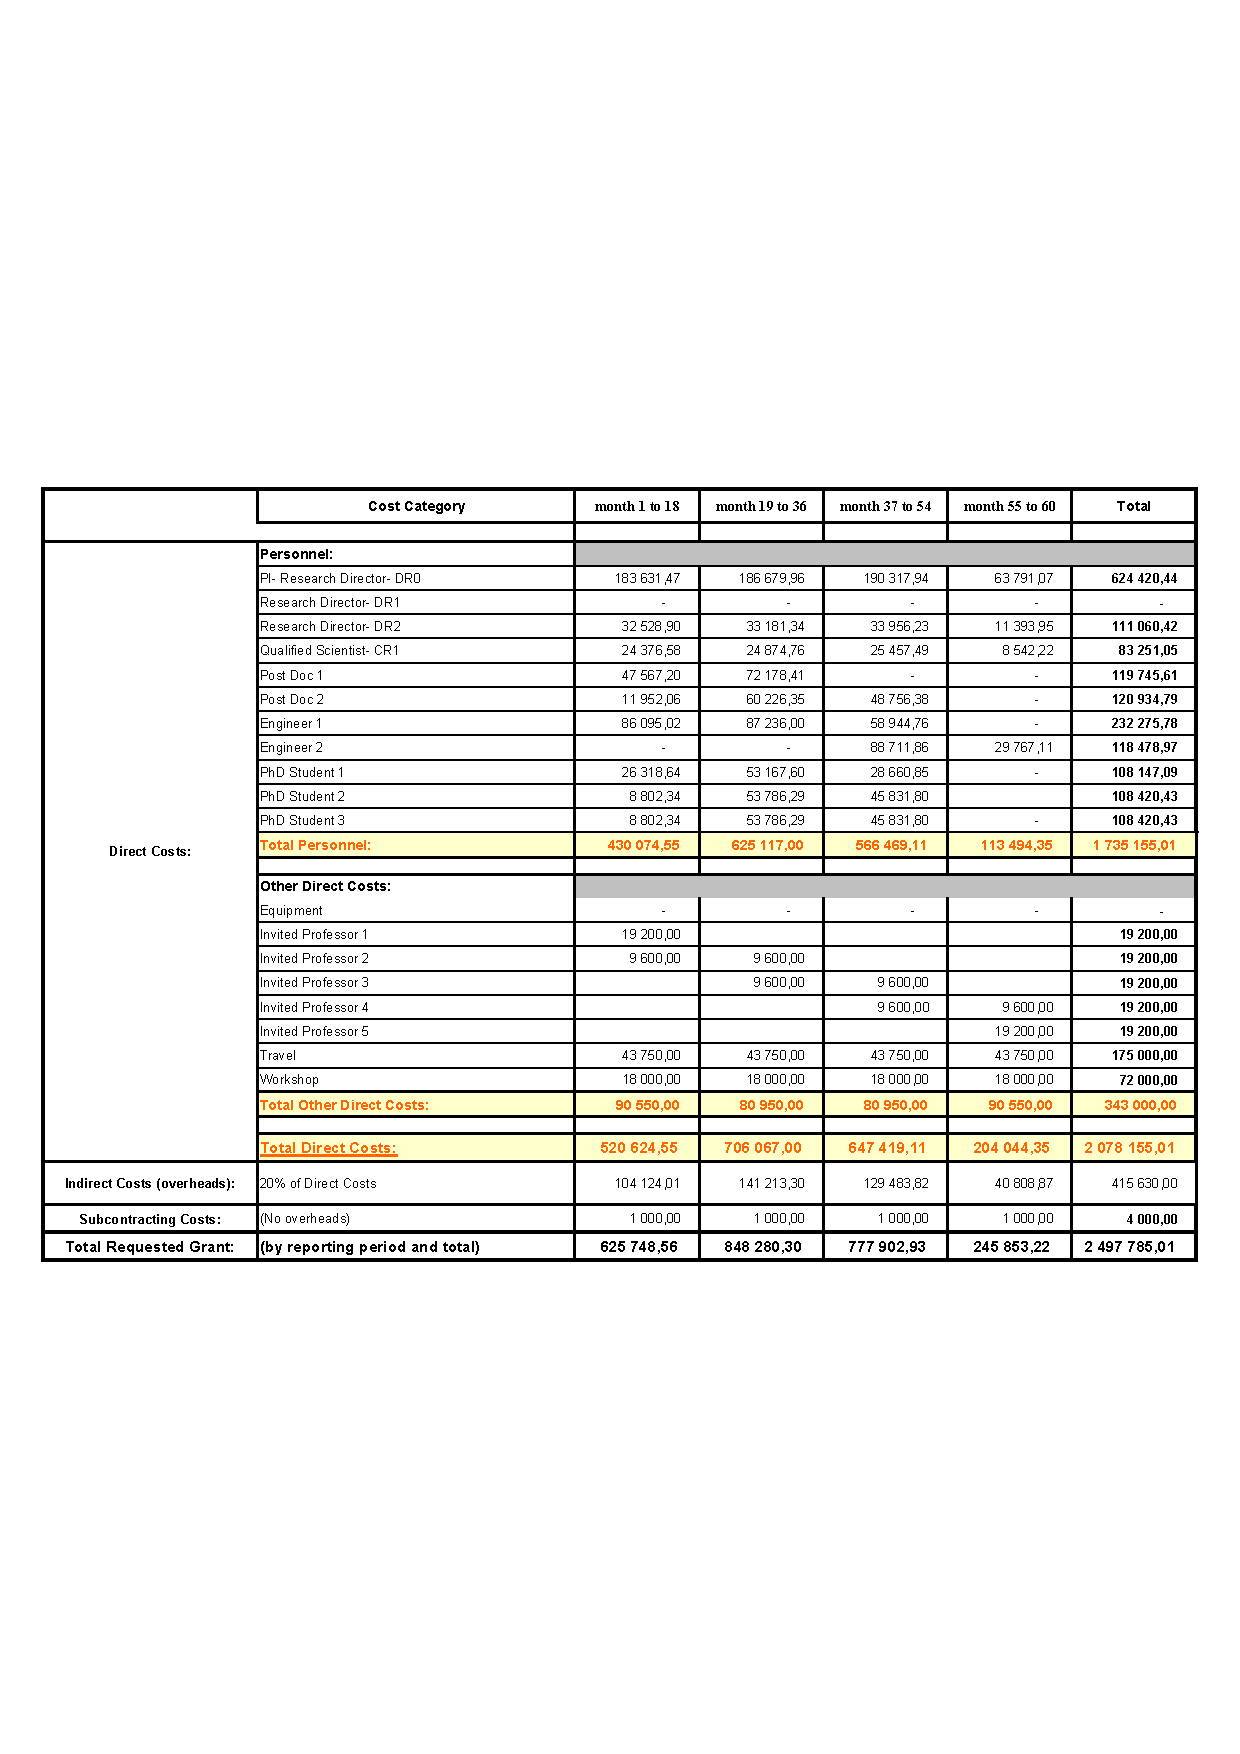
\includegraphics[width=\textwidth]{budget2}


\newpage

{\footnotesize
%\bibliographystyle{alpha}
\bibliographystyle{apalike}
\bibliography{erc}
}

